\section{Implementation}
\label{Imp}

We run modified contiki-ng, a system for next generation IoT (Internet of
Things), on data plane. We modify the network layer of contiki-ng, and abstract
data plane interface to separate network control functions from data plane. 
The details are described as follows.

\textbf{Neighbor Discovery.} After deployment, nodes frist start IPv6 neighbor
discovery protocol to find the nodes which can be reached within one hop, and
then save the neighbor information to neighbor table and wait for UAV arriving
to gather the topology information. Every neighbor's information consists of the
neighbor's IP and RSSI. 

\textbf{Packet forwarding.} The nodes get routing table from UAV through
northbound interface. When a node receive a data packet from other nodes, it
just sends it to the next hop node according the routing table.

\textbf{Data sampling.} Nodes read task table received from UAV to decide when
to wake up sensors to make sure that they cost minimal energy to get the same
quality data. 

\textbf{UAV.} We run our UAV flight controller on ROS (Robot Operating System)
and use MySQL as our SDN database. UAV gathers topology from each node and save
it into database, so that users can easily read the whole network data from
database. For the same reason, after a user gets routing algorithm results and
saves it into database via northbound interface, our control plane will
automatically divides the whole network routing results into individual node's
routing table, and then sends it to specific nodes.

\begin{figure}[htbp]
	\centering
	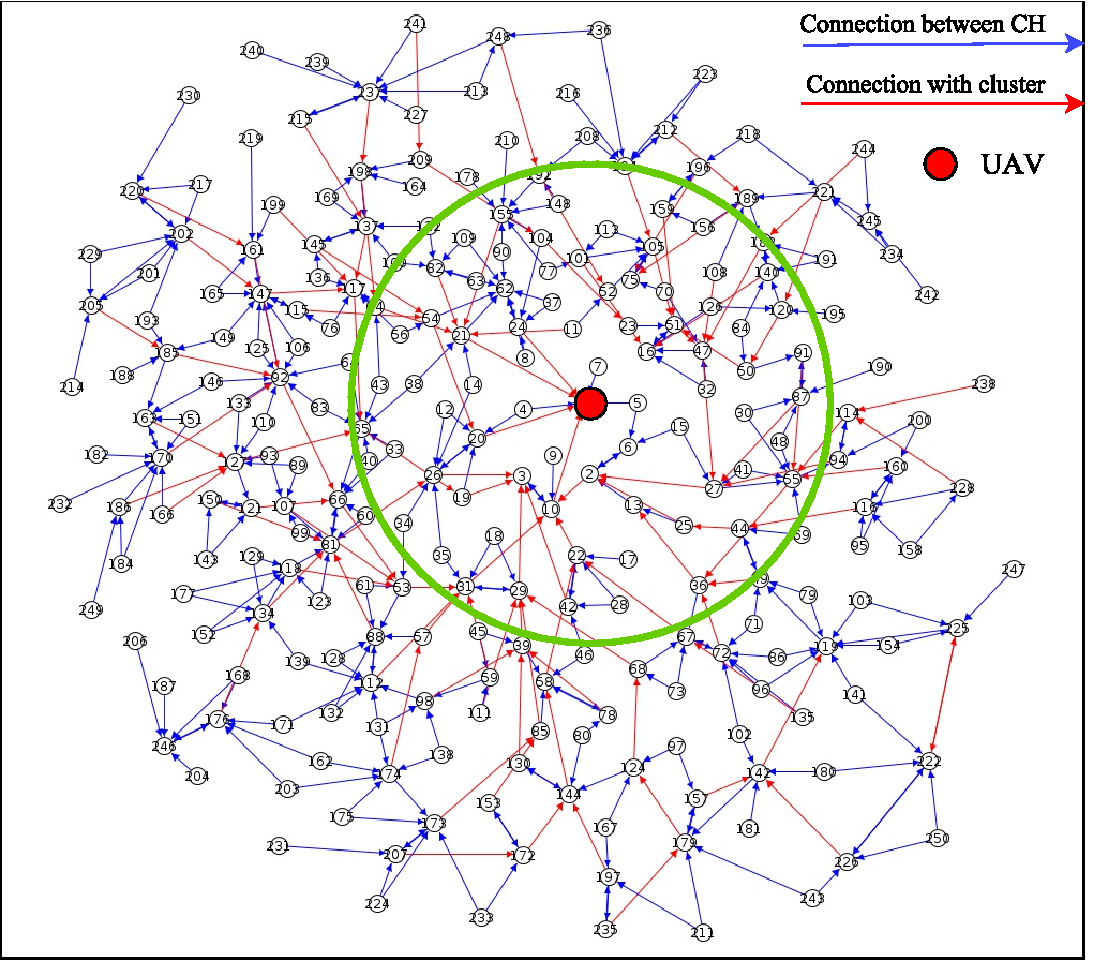
\includegraphics[width=.85\columnwidth]{Figure/topology}
	\vspace{-0.1in}
	\caption{Network topology}
	\label{topology}
	\vspace{-0.1in}
\end{figure}

Based on our software framework, we use DJI M100 UAV with Intel NUC as airborne
computer, and adapt 250 TI CC2650 SensorTag to build our testbed. According to
our UAV gathered topology, we draw Figure~\ref{topology}, the blue lines
represent the connection between cluster members with cluster headers, and the
red lines donate the route between cluster headers deployed by UAV.
